\label{sec:tabellen}
\begin{table}[h!]
\centering
\begin{tabular}{|c|c|}
   	\hline
   	\textbf{Category} &    \textbf{Recall}\\ \hline
   	Capital common countries 	& 0.83202 \\
   	Capital World 				& 0.79134 \\
   	Currency					& 0.35104 \\
   	City in state				& 0.70896 \\
   	Family 						& 0.84585 \\
   	Gram1 adjective to adverb 	& 0.28528 \\
   	Gram2 opposite 				& 0.42734 \\
   	Gram3 comparative 			& 0.90841 \\
   	Gram4 superlative 			& 0.87344 \\
   	Gram5 present participle	& 0.78125 \\
   	Gram6 nationality adjective & 0.89931 \\
   	Gram7 past tense 			& 0.65962 \\
   	Gram8 plural 				& 0.89865 \\
   	Gram9 plural verbs 			& 0.67931 \\
   	\textbf{Total}				& 0.73588 \\ \hline
\end{tabular}
\caption{Word2Vec addition model (ran for 1h15)}
\label{table:word2vec_addition}
\end{table}

\begin{table}[h!]
\centering
\begin{tabular}{| l | c | r}
   	\hline
   	\textbf{Category} &    \textbf{Recall}\\ \hline
   	Capital common countries 	& 0.85178 \\
   	Capital World 				& 0.80570 \\
   	Currency					& 0.35450 \\
   	City in state				& 0.71423 \\
   	Family 						& 0.84585 \\
   	Gram1 adjective to adverb 	& 0.31552 \\
   	Gram2 opposite 				& 0.42365 \\
   	Gram3 comparative 			& 0.90691 \\
   	Gram4 superlative 			& 0.91800 \\
   	Gram5 present participle	& 0.80587 \\
   	Gram6 nationality adjective & 0.89368 \\
   	Gram7 past tense 			& 0.70641 \\
   	Gram8 plural 				& 0.89940 \\
   	Gram9 plural verbs 			& 0.73448 \\
   	\textbf{Total}				& 0.75148 \\ \hline
\end{tabular}
\caption{Word2Vec multiplication model (ran for 3h25)}
\label{table:word2vec_multiplication}
\end{table}

GloVe always had the same amount of skipped words (all words) independent of the dimension within a category. So we will not show the category results for these.

\begin{table}[h!]
	\centering
\begin{tabular}{| l | c | r}
    	\hline
    	\textbf{Category} &    \textbf{Recall}\\ \hline
    	Family 						& 0.85573 \\
    	Gram1 adjective to adverb 	& 0.25403 \\
    	Gram2 opposite 				& 0.22660 \\
    	Gram3 comparative 			& 0.86486 \\
    	Gram4 superlative 			& 0.69786 \\
    	Gram5 present participle	& 0.68277 \\
    	Gram7 past tense 			& 0.60192 \\
    	Gram8 plural 				& 0.77402 \\
    	Gram9 plural verbs 			& 0.59770 \\
    	\textbf{Total}				& 0.30778 \\
    	\textbf{Total no skipped}	& 0.62774 \\ \hline
\end{tabular}
\caption{GloVe50d addition model (ran for 3 min)}
\label{table:glove50d_addition}
\end{table}

\begin{table}[h!]
	\centering
\begin{tabular}{| l | c | r}
    	\hline
    	\textbf{Category} &    \textbf{Recall}\\ \hline
    	Family 						& 0.62846 \\
    	Gram1 adjective to adverb 	& 0.09980 \\
    	Gram2 opposite 				& 0.04926 \\
    	Gram3 comparative 			& 0.41366 \\
    	Gram4 superlative 			& 0.17112 \\
    	Gram5 present participle	& 0.29451 \\
    	Gram7 past tense 			& 0.31153 \\
    	Gram8 plural 				& 0.46021 \\
    	Gram9 plural verbs 			& 0.25862 \\
    	\textbf{Total}				& 0.14506 \\
    	\textbf{Total no skipped}	& 0.29587 \\ \hline
\end{tabular}
\caption{GloVe50d multiplication model (ran for 3 min)}
\label{table:glove50d_addition}
\end{table}


\begin{table}[h!]
	\centering
\begin{tabular}{| l | c | r}
    	\hline
    	\textbf{Category} &    \textbf{Recall}\\ \hline
    	Family 						& 0.81621 \\
    	Gram1 adjective to adverb 	& 0.24395 \\
    	Gram2 opposite 				& 0.20074 \\
    	Gram3 comparative 			& 0.79129 \\
    	Gram4 superlative 			& 0.54278 \\
    	Gram5 present participle	& 0.69508 \\
    	Gram7 past tense 			& 0.55448 \\
    	Gram8 plural 				& 0.71997 \\
    	Gram9 plural verbs 			& 0.58391 \\
    	\textbf{Total}				& 0.28382 \\
    	\textbf{Total no skipped}	& 0.57890 \\ \hline
\end{tabular}
\caption{GloVe100d addition model (ran for 7 min)}
\label{table:glove100d_addition}
\end{table}

\begin{table}[h!]
	\centering
\begin{tabular}{| l | c | r}
    	\hline
    	\textbf{Category} &    \textbf{Recall}\\ \hline
    	Family 						& 0.77866 \\
    	Gram1 adjective to adverb 	& 0.22883 \\
    	Gram2 opposite 				& 0.15764 \\
    	Gram3 comparative 			& 0.74850 \\
    	Gram4 superlative 			& 0.50624 \\
    	Gram5 present participle	& 0.65057 \\
    	Gram7 past tense 			& 0.52821 \\
    	Gram8 plural 				& 0.66667 \\
    	Gram9 plural verbs 			& 0.57356 \\
    	\textbf{Total}				& 0.26668 \\
    	\textbf{Total no skipped}	& 0.54394 \\ \hline
\end{tabular}
\caption{GloVe100d multiplication model (ran for 7 min)}
\label{table:glove100d_addition}
\end{table}



\begin{table}[h!]
	\centering
\begin{tabular}{| l | c | r}
    	\hline
    	\textbf{Category} &    \textbf{Recall}\\ \hline
    	Family 						& 0.85573 \\
    	Gram1 adjective to adverb 	& 0.25403 \\
    	Gram2 opposite 				& 0.22660 \\
    	Gram3 comparative 			& 0.86486 \\
    	Gram4 superlative 			& 0.69786 \\
    	Gram5 present participle	& 0.68277 \\
    	Gram7 past tense 			& 0.60192 \\
    	Gram8 plural 				& 0.77402 \\
    	Gram9 plural verbs 			& 0.59770 \\
    	\textbf{Total}				& 0.30778 \\
    	\textbf{Total no skipped}	& 0.62774 \\ \hline
\end{tabular}
\caption{GloVe200d addition model (ran for 10 min)}
\label{table:glove200d_addition}
\end{table}

\begin{table}[h!]
	\centering
\begin{tabular}{| l | c |}
    	\hline
    	\textbf{Category} &    \textbf{Recall}\\ \hline
    	Family 						& 0.85178 \\
    	Gram1 adjective to adverb 	& 0.25302 \\
    	Gram2 opposite 				& 0.19581 \\
    	Gram3 comparative 			& 0.83784 \\
    	Gram4 superlative 			& 0.67162 \\
    	Gram5 present participle	& 0.67045 \\
    	Gram7 past tense 			& 0.60321 \\
    	Gram8 plural 				& 0.76426 \\
    	Gram9 plural verbs 			& 0.65172 \\
    	\textbf{Total}				& 0.03531 \\
    	\textbf{Total no skipped}	& 0.62273 \\ \hline
\end{tabular}
\caption{GloVe200d multiplication model (ran for 10 min)}
\label{table:glove200d_multiplication}
\end{table}

\begin{table}[h!]
	\centering
\begin{tabular}{| l | c | r}
    	\hline
    	\textbf{Category} &    \textbf{Recall}\\ \hline
    	\textbf{Total}				& 0.31304 \\
    	\textbf{Total no skipped}	& 0.63849 \\ \hline
\end{tabular}
\caption{GloVe300d addition model (ran for 20 min)}
\label{table:glove300d_addition}
\end{table}

\begin{table}[h!]
	\centering
\begin{tabular}{| l | c |}
    	\hline
    	\textbf{Category} 			& \textbf{Recall}\\ \hline
    	\textbf{Total}	  			& 0.32214 \\
    	\textbf{Total no skipped}	& 0.65707 \\ \hline
\end{tabular}
\caption{GloVe300d multiplication model (ran for 20 min)}
\label{table:glove300d_multiplication}
\end{table}

\begin{figure}[ht!]
\centering
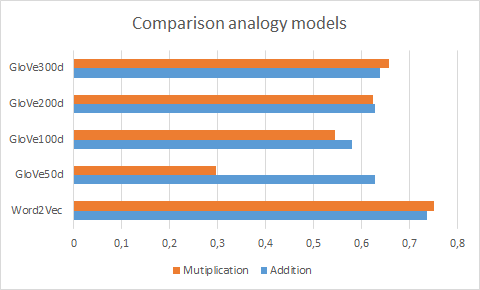
\includegraphics[width=130mm]{images/chart1.png}
\caption{}
\end{figure}
